\section{Overview}\label{sec:overview}

% \begin{figure}
  \begin{subfigure}[c]{\columnwidth}
  \[
    \arraycolsep=3pt\begin{array}{rlrl}
        \text{pattern term} & \spat & ::= &
          \term{\ophole} ~\vert~
          \term{\svar{x}} ~\vert~
          \term{\sparen{\spat}} \\
        & & \vert &
          \term{\spat~\binhole~\spat} ~\vert~
          \term{\sprod{\spat}{\spat}} \\
        \text{expression term} & \sexp & ::= &
          \term{\ophole} ~\vert~
          \term{\snumlit{n}} ~\vert~
          \term{\svar{x}} ~\vert~
          \term{\sparen{\sexp}} \\
        & & \vert &
          % \sap{\sexp}{\sexp} ~\vert~
          \term{\sexp~\binhole~\sexp} ~\vert~
          \term{\sprod{\sexp}{\sexp}} \\
        & & \vert &
          \term{\splus{\sexp}{\sexp}} ~\vert~
          \term{\smult{\sexp}{\sexp}} ~\vert~
          \term{\sdiv{\sexp}{\sexp}} \\
        & & \vert &
          \term{\slam{\spat}{\sexp}} ~\vert~
          \term{\slet{\spat}{\sexp}{\sexp}}
    \end{array}\]
    \caption{}
    \label{fig:term-syntax}
  \end{subfigure}
  \vspace{0.4cm}

  \begin{subfigure}[c]{\columnwidth}
    \[\arraycolsep=3pt\begin{array}{rlrl}
      \text{tile sequence} & \tiles^s & ::= & \tile^s_1\dots\tile^s_n \\
      \text{pattern tile} & \tile^{\pat} & ::= &
        \tophole ~\vert~
        \soptile{\svar{x}} ~\vert~
        \soptile{\sparen{\tiles^{\pat}}} \\
      & & \vert &
        \tbinhole ~\vert~
        \sbintile{\tprod} \\
      \text{expression tile} & \tile^{\expr} & ::= &
        \tophole ~\vert~
        \soptile{\snumlit{n}} ~\vert~
        \soptile{\svar{x}} ~\vert~
        \soptile{\sparen{\tiles^{\expr}}} \\
      & & \vert &
        \tbinhole ~\vert~
        % \sap{}{} ~\vert~
        \sbintile{\tplus} ~\vert~
        \sbintile{\tmult} ~\vert~
        \sbintile{\tdiv} ~\vert~
        \sbintile{\tprod} \\
      & & \vert &
        \spretile{\tlam{\tiles^{\pat}}} ~\vert~
        \spretile{\tlet{\tiles^{\pat}}{\tiles^{\expr}}}
    \end{array}\]
    \caption{}
    \label{fig:tile-syntax}
  \end{subfigure}
  \vspace{0.4cm}
  \caption{
      Term syntax \protect\subref{fig:term-syntax} and tile syntax \protect\subref{fig:tile-syntax}
      for patterns and expressions,
      where
      $x$ ranges over variables
      % $b$ over boolean values,
      and $n$ over number literals.
  }
  \label{fig:term-tile-syntax}
\end{figure}

% \begin{figure}
  \vspace{-3px}
  \[\arraycolsep=3pt\begin{array}{rlrl}
    \text{tile sequence} & \tiles^s & ::= & \tile^s_1\dots\tile^s_n \\
    \text{pattern tile} & \tile^{\pat} & ::= &
      \ophole ~\vert~
      \svar{x} ~\vert~
      \sparen{\tiles^{\pat}} ~\vert~
      \binhole ~\vert~
      \sprod{}{} \\
    \text{expression tile} & \tile^{\expr} & ::= &
      \ophole ~\vert~
      \snumlit{n} ~\vert~
      \svar{x} ~\vert~
      \sparen{\tiles^{\expr}} \\
    & & \vert &
      \binhole ~\vert~
      % \sap{}{} ~\vert~
      \sprod{}{} ~\vert~
      \splus{}{} ~\vert~
      \smult{}{} \\
    & & \vert &
      \slam{\tiles^{\pat}}{} ~\vert~
      \slet{\tiles^{\pat}}{\tiles^{\expr}}{}
  \end{array}\]
  \caption{Tile syntax for patterns and expressions.}
  \label{fig:tile-syntax}
\end{figure}


%\note{could use Alt as toggle indicator}

We now present an example-driven overview of tile-based
editing using \tylr.

\setlength\intextsep{0pt}
\begin{wrapfigure}{r}{0.5\columnwidth}
  \centering
  \texttt{$\boldsymbol{\lambda}$ n \textbf{.} \textbf{(} n , n \textbf{)} , 1}
  \vspace{0.1cm}

  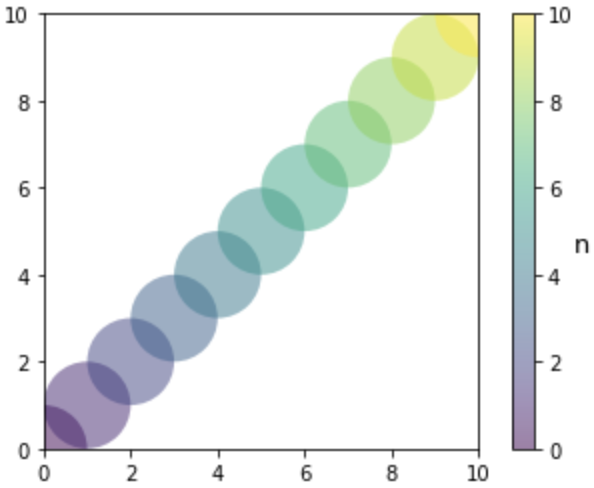
\includegraphics[width=0.5\columnwidth]{img/circles-n-n-1.png}
\end{wrapfigure}
Suppose you are using \tylr~ to edit a function that gets called by a
generative drawing application \cite{sns-pldi}.
\note{use word ``exploratory here''}
The function takes an integer index and
return a circle---represented as a pair comprising
its center point and radius---to be drawn in
the $xy$-plane for every index.
The initial implementation, shown on the right, draws circles
of radius \texttt{1} along the line $y = x$.

\subsection{Tiles}

% \note{maybe forward reference alternative choices not skipping tokens}

Panning your cursor over the program in \tylr ,
as shown in Figure \ref{fig:pan-term-view},
reveals outlined terms of \tylr's concrete syntax,
the relevant subset of which is shown in
Figure \ref{fig:term-syntax}.
\note{for example, the term in the first line of 1c is...}

\note{then transition visually, noting how the term has
separate outline vs highlighted tile, point to tile syntax}

\note{also mention right bias of term view (for simplicity)}

\note{mention tips right away, note hexagon shape}

\note{use lambda example to note how tile syntax is different
from term syntax, noting how lambda tile is actually at
same level of body tiles}

\note{following sentence too vague, couch in concrete example,
be more clear about highlighting the root vs the whole tile,
probably refer explicitly to tile syntax earlier to make it
more precise}
Highlighted at the root of every term is a structure called
a \emph{tile}.
The tile encompasses all tokens used to represent
the root form of the term (e.g., \texttt{1} for a number literal,
$\lambda$ and \texttt{.} for lambda terms,
\texttt{(} and \texttt{)} for parenthesized terms) along with
all children terms delimited on both sides (\eg,
the bidelimited pattern child \texttt{n} of the lambda term,
the bidelimited expression child \texttt{n , n} of
the parenthesized term).
Tiles are color-coded by sort---green for expressions, blue
for patterns---and shaped such that they enclose bidelimited
child terms of different sort and leave unenclosed bidelimited
child terms of the same sort.

\note{need to define sort and bidelimited,
couch this in examination of term syntax}

\begin{figure}
  \centering

   \begin{subfigure}[c]{0.49\columnwidth}
      \centering
      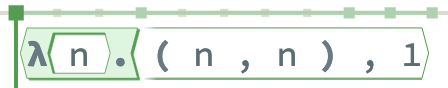
\includegraphics[width=0.9\textwidth]{img/pan-terms-0.png}
      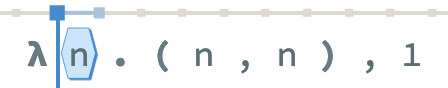
\includegraphics[width=0.9\textwidth]{img/pan-terms-1.png}
      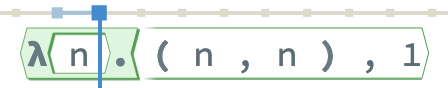
\includegraphics[width=0.9\textwidth]{img/pan-terms-2.png}
      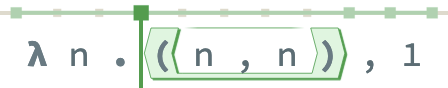
\includegraphics[width=0.9\textwidth]{img/pan-terms-3.png}
      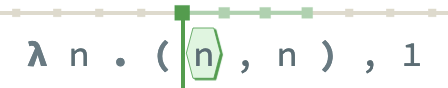
\includegraphics[width=0.9\textwidth]{img/pan-terms-4.png}
      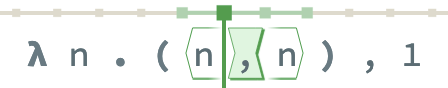
\includegraphics[width=0.9\textwidth]{img/pan-terms-5.png}
      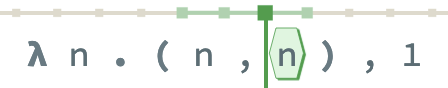
\includegraphics[width=0.9\textwidth]{img/pan-terms-6.png}
      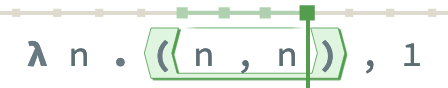
\includegraphics[width=0.9\textwidth]{img/pan-terms-7.png}
      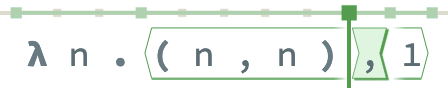
\includegraphics[width=0.9\textwidth]{img/pan-terms-8.png}
      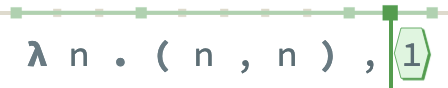
\includegraphics[width=0.9\textwidth]{img/pan-terms-9.png}
      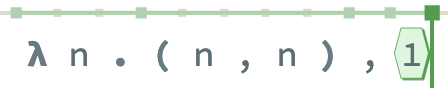
\includegraphics[width=0.9\textwidth]{img/pan-terms-10.png}
      \caption{}
      \label{fig:pan-term-view}
  \end{subfigure}
  \begin{subfigure}[c]{0.49\columnwidth}
    \centering
    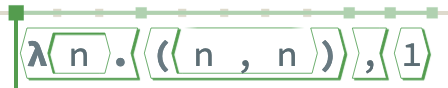
\includegraphics[width=0.9\textwidth]{img/pan-tiles-0.png}
    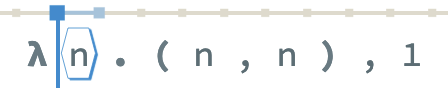
\includegraphics[width=0.9\textwidth]{img/pan-tiles-1.png}
    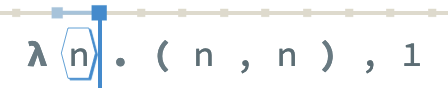
\includegraphics[width=0.9\textwidth]{img/pan-tiles-2.png}
    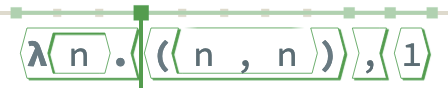
\includegraphics[width=0.9\textwidth]{img/pan-tiles-3.png}
    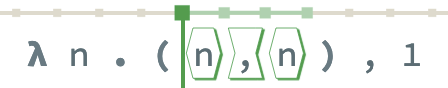
\includegraphics[width=0.9\textwidth]{img/pan-tiles-4.png}
    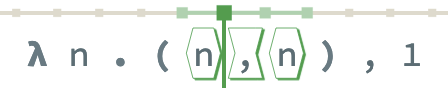
\includegraphics[width=0.9\textwidth]{img/pan-tiles-5.png}
    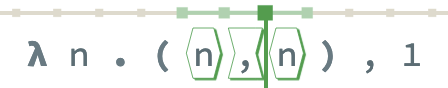
\includegraphics[width=0.9\textwidth]{img/pan-tiles-6.png}
    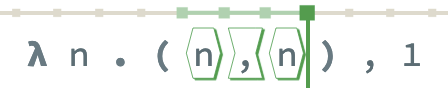
\includegraphics[width=0.9\textwidth]{img/pan-tiles-7.png}
    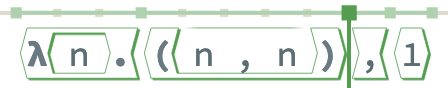
\includegraphics[width=0.9\textwidth]{img/pan-tiles-8.png}
    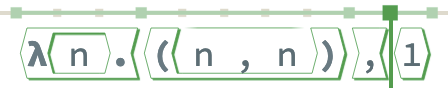
\includegraphics[width=0.9\textwidth]{img/pan-tiles-9.png}
    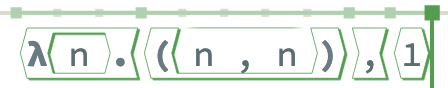
\includegraphics[width=0.9\textwidth]{img/pan-tiles-10.png}
    \caption{}
    \label{fig:pan-tile-view}
  \end{subfigure}
  \vspace{10pt}
  % \end{minipage}
  \caption{\tylr's pointing mode in \protect\subref{fig:pan-term-view} term view
  and \protect\subref{fig:pan-tile-view} tile view }
  \label{fig:pan}
\end{figure}


Tiles are shaped at their ends to fit together sequentially
into operator sequences.
% \begin{align*}
% \langle\overline{\underline{\text{operand}}}\rangle,
% \langle\overline{\underline{\text{prefix operator}}}\langle, \\
% \rangle\overline{\underline{\text{postfix operator}}}\rangle,
% \rangle\text{infix operator}\langle.
% \end{align*}
Holding Alt/Option at any time reveals the local tile sequence
housing the cursor, as shown in Figure \ref{fig:pan-tile-view}.
Where other structure editors model their edit states
using the strictly hierarchical term syntax,
\tylr~ instead models its edit state
using the flattened tile syntax, parsing the tile structure
as needed to produce the term structure.
Indeed, the apparent term structure shown in Figure
\ref{fig:pan-term-view} is simply a
decoration overlaid atop the actual tile structure shown in
Figure \ref{fig:pan-tile-view}.

\note{add discussion of tile structure well-formedness,
discuss sort-colored cursor positions}

\note{need to define pointing mode}

\note{mention holes, forward reference how these will
be key players moving forward, explicitly mention
the convex contiguity of well-formed opseqs}

% Tiles are closely related to nested words \note{cite} and
% visibly pushdown languages \note{cite}, which we discuss
% further in Section \ref{sec:related-work}.

\subsection{Inserting tiles}
By having you edit the tile structure, and only
indirectly propagate those edits to the term structure,
\tylr~ recovers many of the flexible editing affordances to
which you are accustomed in a text editor.

\paragraph{Linear construction of operator sequences}
For example, say you update the function to
draw circles along the parabola $y = x^2/9$,
accomplished via the following edit sequence:

\noindent
\begin{minipage}[t]{0.2\columnwidth}
  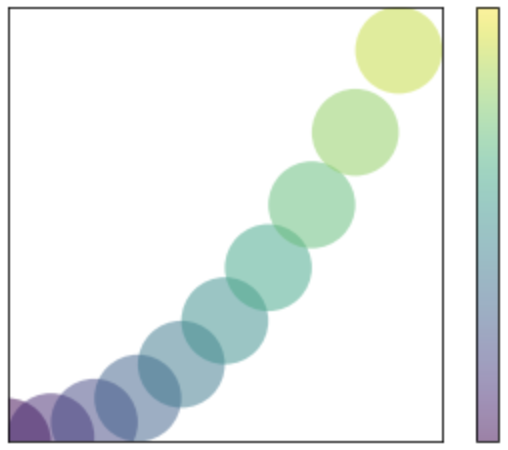
\includegraphics[width=\textwidth]{img/circles-parabola.png}
\end{minipage}
\hfill
\begin{minipage}{0.65\columnwidth}
  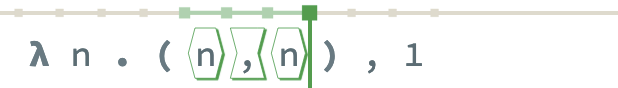
\includegraphics[width=\textwidth]{img/linear-insertion-0.png}
  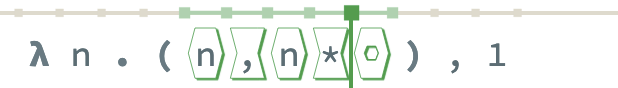
\includegraphics[width=\textwidth]{img/linear-insertion-1.png}
  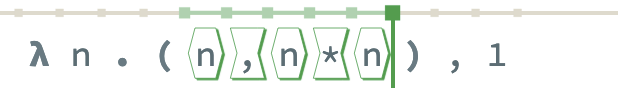
\includegraphics[width=\textwidth]{img/linear-insertion-2.png}
  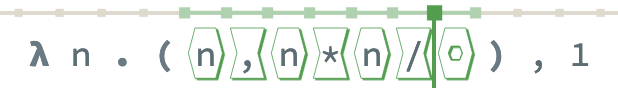
\includegraphics[width=\textwidth]{img/linear-insertion-3.png}
  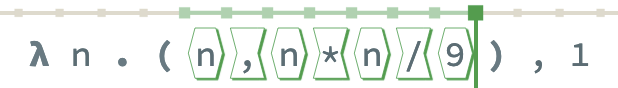
\includegraphics[width=\textwidth]{img/linear-insertion-4.png}
\end{minipage}

\note{add one more final snapshot in term view, showing
how tylr parses precedence/associativity}

\note{pause after constructing the times and note how
precedence is re-parsed}

You constructed the operator sequence \texttt{n * n / 9}
by typing left-to-right, as you might in a text editor, without any
required consideration for its tree structure.
Such an affordance is not trivial
in traditional structure editors because,
from the perspective of the AST, linear construction of
operator sequences is a complex, context-sensitive operation.
Existing structure editors either embrace strictly tree-based
construction of operator sequences;
defer to text at the expression level,
recovering linearity at the cost of structure;
or solve the problem at the cost of complexity
(e.g. side transforms in MPS).
Tiles enable linear editing of operator sequences,
while continuously maintaining structure and
relying on simple precedence parsing
to update the operator sequence's associative structure
as you type.

\note{note that this is insertion, not ``hole filling'' as
it is traditionally conceived in structure editors}

\note{figure out way to say wholesale but not being whole program}

\note{insert a comment somewhere about no performance claims}

\note{review side transforms and make sure I'm not BSing}


\note{figure out where to talk about hole insertion based on tips
somewhere here}

% \tylr~ takes a different approach to this problem.
% Where traditional structure editors simply expose editing
% operations acting directly on the abstract syntactic struture
% of a program, \tylr~ presents the program in a separate
% concrete syntax with its own syntax-directed editing operations.
% \note{
%   talk about tile syntax show in Figure \ref{fig:tile-syntax},
%   note linearity
% }
% Like text, \tylr's concrete syntax gives you ``flattened''
% representation of your program that can be edited in a linear fashion.
% Unlike text, the concrete syntax maintains hierarchies of
% bidelimited children and can always be parsed into
% the abstract syntax, provided that the structure first undergoes
% a hole fixing pass in which holes are inserted and removed
% as needed. \note{need more context about tiles + bidelimited, bring
% back some old words about abstract syntactic structural units
% as opposed to concrete syntactic structural units}

% \note{perhaps go back to editor syntax terminology}

\begin{figure*}
  \begin{tabular}{cp{0.7\textwidth}}
  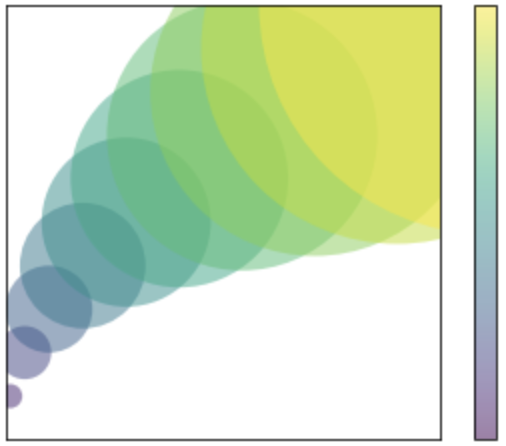
\includegraphics[width=0.1\textwidth]{img/circles-parabola-grow-1.png}
  &
  {
    \begin{align*}
      & \texttt{$\lambda$ n . let x , y = \_|in ( n * n / 9 , n ) , 1} \\
      & \texttt{$\lambda$ n . let x , y = \_|in|( n * n / 9 , n ) , 1} \\
      & \texttt{$\lambda$ n . let x , y = [in]( n * n / 9 , n ) , 1} \\
      & \texttt{$\lambda$ n . let x , y = ( n * n / 9 , n )[in], 1} \\
      & \texttt{$\lambda$ n . let x , y = ( n * n / 9 , n )|in \_ , 1} \\\\
      & \texttt{$\lambda$ n . let x , y = ( n * n / 9 , n|) in x , y , 1 } \\
      & \texttt{$\lambda$ n . let x , y = ( n * n / 9 , n|)|in x , y , 1 } \\
      & \texttt{$\lambda$ n . let x , y = |(|n * n / 9 , n[)]in x , y , 1 } \\
      & \texttt{$\lambda$ n . let x , y = |(|[)]n * n / 9 , n in x , y , 1 } \\
      & \texttt{$\lambda$ n . let x , y = [(][)]n * n / 9 , n in x , y , 1 } \\
      & \texttt{$\lambda$ n . let x , y = n * n / 9 , n in [(][)]x , y , 1 } \\
      & \texttt{$\lambda$ n . let x , y = n * n / 9 , n in ( x , y[)], 1 } \\
      & \texttt{$\lambda$ n . let x , y = n * n / 9 , n in ( x , y|) , 1 } \\\\
      & \texttt{$\lambda$ n . let x , y = n * n / 9 , n in ( x , y ) ,|x + y } \\
      & \texttt{$\lambda$ n . let x , y = n * n / 9 , n in ( x , y ) ,|(|[)]x + y } \\
      & \texttt{$\lambda$ n . let x , y = n * n / 9 , n in ( x , y ) ,|(|x + y[)]} \\
      & \texttt{$\lambda$ n . let x , y = n * n / 9 , n in ( x , y ) , ( x + y|)} \\
      & \texttt{$\lambda$ n . let x , y = n * n / 9 , n in ( x , y ) , ( x + y )|} \\
      & \texttt{$\lambda$ n . let x , y = n * n / 9 , n in ( x , y ) , ( x + y ) /|\_} \\
      & \texttt{$\lambda$ n . let x , y = n * n / 9 , n in ( x , y ) , ( x + y ) / 4|}
    \end{align*}
  }
  \end{tabular}
\end{figure*}

\begin{figure*}
  \begin{tabular}{cp{0.7\textwidth}}
  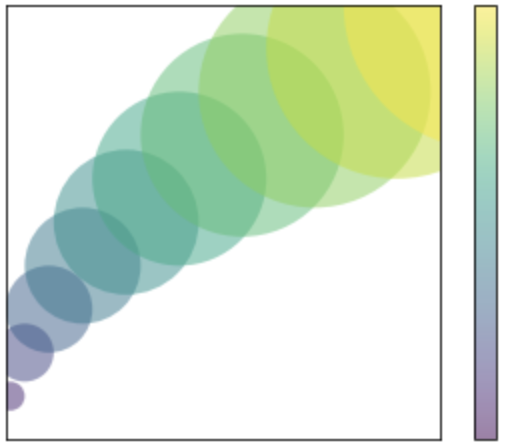
\includegraphics[width=0.1\textwidth]{img/circles-parabola-grow-2.png}
  &
  {
    \begin{align*}
      & \texttt{$\lambda$ n . let x , y = n * n / 9 , n|in ( x , y ) , n / 3} \\
      & \texttt{$\lambda$ n .|let x , y =|n * n / 9 , n[in] ( x , y ) , n / 3} \\
      & \texttt{$\lambda$ n . n * n / 9 , n|\_ ( x , y ) , n / 3} \\
      & \texttt{$\lambda$ n . n * n / 9 , n \_ (|x , y ) , n / 3} \\
      & \texttt{$\lambda$ n . n * n / 9 , n \_ (|x , y|) , n / 3} \\
      & \texttt{$\lambda$ n . n * n / 9 , n \_ (|\_ ) , n / 3} \\
      & \texttt{$\lambda$ n . n * n / 9 , n [(]|)|, n / 3} \\
      & \texttt{$\lambda$ n .[(]n * n / 9 , n|)|, n / 3} \\
      & \texttt{$\lambda$ n .|( n * n / 9 , n ), n / 3}
    \end{align*}
  }
  \end{tabular}
\end{figure*}

\subsection{Selecting and restructuring}
Tiles not only simplify linear \emph{insertion} in a structured
context but also enable text-like \emph{selecting}
and \emph{restructuring} (e.g. cut and paste) of existing code.
While the former problem is relatively well-studied
\note{cite MPS, modeless structure editing},
almost no attention has been paid to the latter.
In particular, all prior structure editors restrict
structured selections to complete concrete syntactic terms,
a severe limitation compared to the arbitrary range
selections of text editors.

\tylr~ recovers much of this lost flexibility.
Using \tylr's \emph{selecting mode}, you can
make arbitrary range selections up to token boundaries,
disassembling tiles into \emph{shards} as needed.
Using \tylr's \emph{restructuring mode},
you can pick up your selections into your
\emph{backpack} and put them down elsewhere,
à la cut-and-paste using the clipboard.
Unlike the usual clipboard, however,
your backpack is structure-aware and guides your
movement toward valid paste targets, \ie,
you can only put down your backpack's contents
where the result can be reassembled into well-formed tiles.

\note{add another paragraph header focused on selecting}

\note{see if I can talk about intact vs cracked selections here,
perhaps by changing the direction of the first selection and
introducing shards when right parens get selected}

\note{so far we have been in pointing mode...}

\paragraph{Restructuring with a full backpack}
Say you update your circle drawing
to its transposition, i.e., draw the circles along
the parabola $x = y^2/9$.
Entering selecting mode, you anchor the selection's right
end and move left to select the tiles you just
inserted in the $y$-coordinate---an impossible
selection in prior structure editors.

\noindent
\begin{minipage}[t]{0.2\columnwidth}
  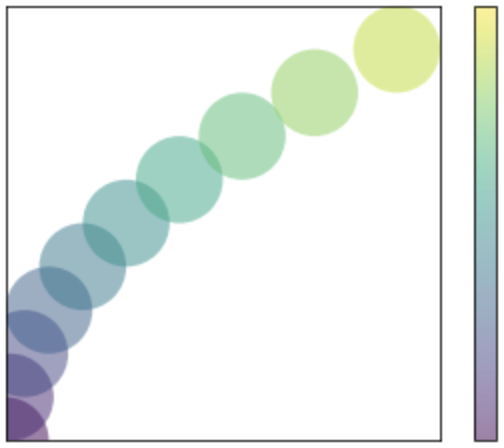
\includegraphics[width=\textwidth]{img/circles-parabola-transpose.png}
\end{minipage}
\hfill
\begin{minipage}{0.65\columnwidth}
  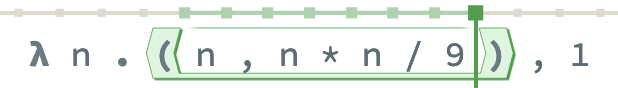
\includegraphics[width=\textwidth]{img/selection-whole-0.png}
  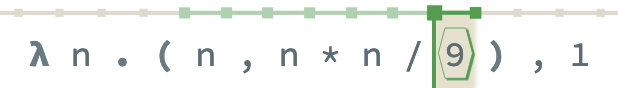
\includegraphics[width=\textwidth]{img/selection-whole-1.png}
  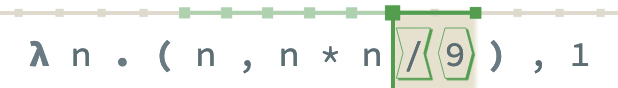
\includegraphics[width=\textwidth]{img/selection-whole-2.png}
  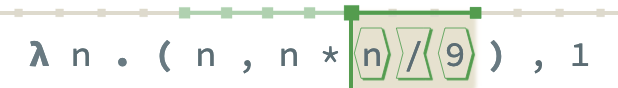
\includegraphics[width=\textwidth]{img/selection-whole-3.png}
  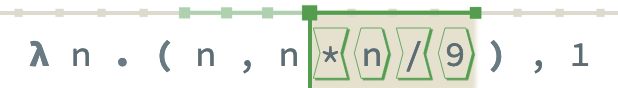
\includegraphics[width=\textwidth]{img/selection-whole-4.png}
\end{minipage}
You then pick it up into your backpack to enter
restructuring mode.
Moving left to the $x$-coordinate and putting down
the selection completes the desired transformation.

\noindent
\begin{tabular}{cp{7cm}}
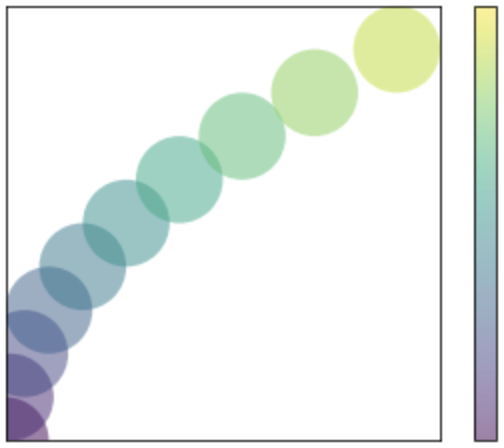
\includegraphics[width=2cm]{img/circles-parabola-transpose.png}
&
{
\begin{align*}
  & \texttt{$\lambda$ n . ( n , n[* n / 9]) , 1} \\
  & \texttt{$\lambda$ n . ( n ,[* n / 9]n ) , 1} \\
  & \texttt{$\lambda$ n . ( n[* n / 9], n ) , 1} \\
  & \texttt{$\lambda$ n . ( n|* n / 9 , n ) , 1}
\end{align*}
}
\end{tabular}

\note{define intact selections}

We say that your backpack is \emph{full} whenever
its contents are, or can be assembled into, whole tiles.
If your backpack is full, then you may move freely,
since you may insert a selection of whole tiles anywhere and
still have a valid nested tile structure.
\tylr~ would have prevented you from putting
down your selection of expression tiles in a pattern
position; we discuss sort conversions in Section ??.
\note{awkward ending}

\note{define cracked selections}

Often, however, your backpack's contents are not whole
tiles, nor can they be assembled into tiles.
In that case, we say that your backpack is \emph{hungry}.

\paragraph{Restructuring with a hungry backpack}

\note{add back brief paragraph describing constructing let tile,
compress into single row in edit sequence}

Say now you would like the circles' radii to grow
with their origin coordinates; accordingly,
as shown at the top of Figure ??,
you have inserted
a let tile introducing variables \texttt{x} and \texttt{y}
in the function body.
Your remaining task is to restructure your code so that \texttt{x}
and \texttt{y} are bound to the origin coordinates
\texttt{( n * n / 9 , n )} currently in the body of the let term.
You begin by selecting the \texttt{in} delimiter,
which disassembles the \texttt{let}-tile into a pair of \emph{shards}.
You then pick up the \texttt{in} shard into your backpack,
move right once, and put it down,
upon which \tylr~ reassembles the \texttt{let}-tile
and returns you to pointing mode.

\note{figure out a way to introduce hole fixing, why operand hole
disappears rather than operator hole being introduced, might be
here or worked in before}

\note{when discussing hole minimality, distinguish from other
interfaces where you insert holes manually, so you shouldn't
remove automatically}

% Your editing workflow was similar to what you might
% have done in a text editor---delete the \texttt{in}
% delimiter, move right, re-type---except that \tylr~
% skipped all cursor positions within the parentheses tile
% when you moved right.
Notice that you skipped all cursor positions within
the parentheses tile when you moved right.
The \texttt{in} shard in your backpack cannot be assembled into
a whole tile on its own, meaning at least one matching shard---in
this case, \texttt{let x , y =}---is
anchored within the current tile sequence.
This restricts your movement of the \texttt{in}
shard to cursor positions of the same sequence,
as placing it in any other position would
violate proper tile nesting on reassembly.
\note{say something explicitly of the form "when your backpack
is hungry... blah blah"}


\note{add back some discussion comparing to text editing
and other structure editors;
similarity with text workflow,
while making it more efficient + less cognitive load;
other structure editors would force you to translate
edits into term-based selections, can be awkward or
not the most efficient in terms of selection size}

We call your backpack full or hungry as a way
to narrativize its control of your movement.
When your backpack is full, it is satisfied
and lets you move freely and leisurely through
your code.
When your backpack is hungry, it accelerates your
movement through the current tile sequence
in impatience to end its hunger, which can happen in one of two ways.
Either, like in the last example, you can empty your backpack,
freeing it of all earthly possessions and desires;
or you may feed it.

\note{add forward reference to discussing alternatives, eg,
not skipping cursor positions}

% We hypothesize that such a restriction would lead to both greater
% editing efficiency and reduced cognitive load compared to
% text editing on similar tasks.

% We hypothesize that such a restriction would easy to learn
% given
% \begin{itemize}
% \item be easy to learn, given the workflow similarity to text editing;
% \item lead to greater editing efficiency than text editing due to
%     the fewer keypresses needed to reach valid paste/restructure targets; and
% \item reduce cognitive load compared to text editing because you
%     no longer need to count delimiters to ensure you have reached
%     a valid paste/restructure target.
% \end{itemize}

\paragraph{Feeding your hungry backpack}
Say you have filled the hole in Figure ?? with
the variables \texttt{x} and \texttt{y} you defined
in the previous example, as shown in Figure ??.
Upon reviewing the term structure, however, you
discover that pairs are right-associative in \tylr,
so you need to wrap \texttt{x , y} in parentheses
in order to satisfy the expected return type.
\note{maybe just say we've created a triple but we
really want a pair of a pair on left}
You also notice that the parentheses in the definition
of the \texttt{let} tile are now redundant
and decide to recycle them.
You move your cursor to the right parenthesis,
select it, and pick it up into your backpack.
At this point your backpack is hungry and restricts
your movement to the tile sequence within the
let definition.
Instead of emptying your backpack like in the
last example, this time you move over to the
left parenthesis and pick it up as well (Figure ??).

\note{make note of pattern not having parentheses}

% When your backpack carries multiple selections,
% it dictates the order in which you can put them down.
% Most of the time it behaves like a stack, putting
% down first the last picked up selection; we discuss
% deviations

Now your backpack is full, as it carries both shards
needed to assemble a whole parenthesis tile,
and you may move freely again.
You carry the parentheses over to the body of the
let term and wrap \texttt{x , y} to complete your
restructuring.

The last example showed how \tylr~ lets you carry \emph{multiple}
related range selections in your backpack.
This ability vastly improves your selecting precision
compared to prior designs.
From the perspective of the term syntax,
where other structure editors force you to select
complete subtrees, \tylr~ lets you cut out individual
\emph{nodes} of the tree and splice them back in
elsewhere.
\note{either remove this or rewrite when it's more as
an emergent phenomenon}

\paragraph{Staging tile insertion}
\note{maybe just call restructuring on insertion}

\note{add connecting intro connecting to node-centric perspective}
Say you have completed an initial draft of your goal program,
where each circle's radius is the sum of its origin
coordinates, as shown in Figure ??.
You discover, however, that the circles are so large that
they fill your viewport, so you would like to make them smaller.
You begin by inserting a left parenthesis
before \texttt{x + y}, your intention being to wrap
the sum and divide it by a constant factor.
Upon this insertion, \tylr~ automatically enters
restructuring mode with the matching right parenthesis
in your backpack.
You move right, put down the right parenthesis,
and complete your desired transformation.

\note{add discussion}

\note{note how other structure editors force you to select
child first before constructing}


\paragraph{Picky eater}
We call the cursor positions marking the ends of a selection
the selection's \emph{caps}.
So far we have only encountered selections with caps
of the same sort.
Your backpack is a ``picky eater'' in that
it will refuse to carry any selections with caps of
different sort.

Consider, for example, the following selection:

\note{example fig}

\noindent
The left cap is pattern-sorted while the right cap
is expression-sorted, as indicated by the two-toned
broken overline.
Picking up this selection would bring together
tiles of different sort, violating \tylr's edit
state well-formedness, so you are prevented from doing so.

\note{show small inline example of selecting
selection with caps of different sort}

\note{show small inline example of selection
with pattern caps cutting across expressions}

\subsection{Removing selections}
Finally, we turn our attention to removal.
Removing a selection works in one of two ways,
depending on whether your selection is intact or fragmentary.

\paragraph{Removing intact selections}
Say you fiddled some more with your last circle drawing
and discovered a similar drawing you like a bit better,
shown in Figure ??.
Upon reviewing your code, you realize you no longer
need to define variables \texttt{x} and \texttt{y},
since they are each used only once, and can inline
their definition.
You begin by removing the uses of \texttt{x} and \texttt{y},
selecting \texttt{x , y} in the body of the \texttt{let}
term and hitting Backspace.
In this case, because your selection is intact, \tylr~
immediately removes your selection, as you might
expect from your experience with text editors.

\paragraph{Removing fragmentary selections}
Now you would like to remove the \texttt{let} tile,
but you want to preserve its definition so you
can inline it.
You select the \texttt{in} shard and hit Backspace.
Because your selection is fragmentary, removing
your selection would require also removing the
matching \texttt{let} shard that you have not
explicitly selected yourself.
\note{something about removal at a distance, also
mention prior designs here}
\tylr~ does not remove both shards immediately, but
instead enters restructuring mode as a staging ground
in which you are shown explicitly the affected
selections.
\note{referencing back to restructuring we've already seen,
which then gives you the option to...}
You confirm the total removal by hitting Backspace again,
leaving behind the let definition and body expressions
separated by an operator hole.

In general, pressing Backspace on a selection
has one of two effects:
\begin{enumerate}
  \item[(1)] remove the selection if it is intact
    and return to pointing mode;
  \item[(2)] otherwise entering restructuring mode with
    the smallest containing selection with same-sort caps
    in your backpack.
\end{enumerate}
Pressing Backspace again in restructuring mode
removes all highlighted tiles and selections.
In sum: if your selection is intact then you can
remove it with a single tap of Backspace; otherwise
you need to double tap.

% If your selection is fragmentary, then removing
% your selection would require also removing matching shards
% that you have not explicitly selected yourself.
% \tylr~ does not remove the implicit selections immediately
% but instead enters restructuring mode as a staging
% ground in which you may confirm the total removal
% by hitting Backspace again (or otherwise proceed
% with restructuring).
\note{draw parallel with staged insertion}
% In sum: if your selection is intact then you can
% remove it with a single tap of Backspace; otherwise
% you need to double tap.


\paragraph{Removing in pointing mode}
Finally, it remains to restructure the parentheses
so that they wrap the origin coordinates.
This time, instead of first explicitly specifying a selection,
you position your cursor after the left parenthesis
and hit Backspace within pointing mode.
\tylr~ treats this input simply as a shortcut for selecting the
token immediately to your left and then hitting Backspace.
In this case, the token to your left is a parenthesis
shard that forms a fragmentary selection, so you
enter restructuring mode with the parenthesis in tow.
You move left to the other side of the origin coordinates,
then put down the parenthesis to complete the transformation.

\vspace{0.5cm}

\note{rework following so it's \tylr-centered,
talk about how \tylr~ improves on deletion in other editors}


which warrants first a preliminary critique of how it
works in existing term-based editors.

As with selection, term-based editors typically
limit delete operations so they can only act on
complete terms, which can force preemptive and tedious
maneuvering to prevent excessive removal.
For example, removing a block in a block-based editor
removes all of its descendant blocks as well.
If you intended only to delete a specific block
while preserving its descendants, you are forced
to save its children first by moving them elsewhere
before you can actually delete the block.
JetBrains MPS, a mature text-like structure editor,
mitigates this by preserving the first child of a deleted term
if they happen to share the same sort,
but cannot preserve more than one child in a generic
structure-preserving way.

Meanwhile, it can be difficult to predict the
effects of term-based deletion in a text-like
interface, like MPS, that provides less visual
indication of term structure than a block-based editor.
Consequently a delete operation can be much
more destructive than expected, \eg,
pressing Backspace on a token
causes a large containing range to disappear.
Indeed, a (controlled) user study of MPS revealed
that even \emph{experts} feel that deletion in MPS
is relatively inaccurate (compared to corresponding
subjective assessments made by text editor users),
which we interpret to mean they have difficulty
predicting its behavior.


Tile-based editing reduces the destructive effect of deletions
compared to term-based editing; moreover \tylr~ explicitly
highlights everything that will be removed upon your deletion
so that you never have to guess or reason through it.

\note{discuss a bit following a text editing like flow as much
as possible, but using restructuring to guide you in cases
where you can't just do the text thing}

\note{acknowledge sort-based limitations of tile structure
in limitation section, possibly mention statements, lean into
our philosophy but here are some thoughts}

%\note{consider doing insertion, selection, deletion, then
%restructuring as a better progression}


% \subsection{\note{everything below this is old overview}}

% Tile-based structure editing departs from traditional
% structure editors in avoiding direct user modifications
% to the AST.
% Instead, much like with a text editor, the user modifies a separate
% ``flattened'' editing structure that affords more flexible
% editing mechanisms, which is subsequently parsed into the
% abstract syntax.
% Unlike a text editor, however, a tile-based editor ensures
% that every edit state can be parsed successfully.

% In this section we motivate and give an example-driven
% overview of tile-based editing as implemented
% in \tylr. We begin by describing the limitations of
% traditional structure editors, then show how tile-based
% editing overcomes these limitations.

% \subsection{A typical structure editor} \label{sec:simple-editor}

% Structure editors, also known as projectional editors, typically
% follow a projectional architecture: the editor projects an
% abstract syntax tree into a concrete representation,
% and user interactions with the representation are interpreted
% by the editor as direct modifications to the AST.

% For example, suppose we wish to edit expressions with the abstract
% syntax presented in Figure \ref{fig:tile-syntax}.
% A simple editor might project the current expression
% to a textual notation decorated with nested boxes, such
% that there is a one-to-one correspondence between
% boxes and terms. \note{example}
% In this editor, the cursor selects a subterm of the
% current program expression and may be moved through
% the current expression via a pre-order traversal.
% Edits are context-free transformations
% of the selected subterm:
%   deletion replaces the current subterm with
%     a hole of the same sort; and
%   construction replaces the current subterm
%     with the new form, making the original subterm
%     a child of the new form if possible, and moving
%     the cursor to the next child position if available.

% While simple, this editor is representative of existing structure
% editors in the way that it restricts editing affordances to easily
% understood tree manipulations of the abstract syntax.
% We believe such restrictions unacceptably hamper usability.
% Consider the following classes of edits that we may wish to
% perform---and could perform in a text editor---but cannot with the
% given interface:

% \paragraph{Linearly constructing operator sequences}
% In a text editor, we may type the characters \texttt{2}, \texttt{*},
% \texttt{3}, \texttt{+}, \texttt{4}
% to construct the expression \texttt{2 * 3 + 4} with
% the usual precedence-based operator associations.
% In our simple structure editor, the same inputs would construct
% the following series of edit states: \note{todo figure}.
% To get the associations we want, we would need to interleave
% our constructions with movements through the expression tree
% to ensure that the correct child is chosen before constructing
% the plus node: \note{todo figure}.
% This particular limitation of structure editing is well-recognized
% in prior work, which we discuss in greater detail in Section
% \ref{sec:related-work}.

% \paragraph{Preserving children of deleted terms}
% Deletion in our simple editor is quite coarse, deleting whole
% trees rather than individual nodes.


% \begin{itemize}
% \item
%   we now describe a few classes of edits that we may wish to perform---and
%   could perform in a text editor---but cannot with the given structured
%   interface
% \item structure-oblivious linear construction of operator sequences
%   \begin{itemize}
%     \item eg going from \texttt{2 * 3 + 4} as opposed to \texttt{2 * (3 + 4)}
%     \item this particular limitation of naive structure editing has received
%       the most attention in prior work
%     \begin{itemize}
%       \item some structure editors defer to text at the leaves
%       \item others develop more sophisticated methods, e.g.,
%         modeless structure editing article,
%         MPS's side transforms
%     \end{itemize}
%   \end{itemize}
% \item deleting the root of a term,
%   leaving behind its children for further processing
%   (eg splicing into the surrounding context)
%   \begin{itemize}
%     \item eg it is not possible to delete a let expression and leave behind its body
%     \item eg it is not possible to remove a conditional expression
%       and leave behind a branch to take its place, or to subsequently join the
%       two remaining branches with an operator
%     \item note how there's no room in the strict tree structure to deal with
%       multiple "floating" children
%     \item MPS mitigates this by leaving behind its first child if its the
%       same sort, but already this does not satisfy the use case described above,
%       and in general the user should have the freedom to choose
%   \end{itemize}
% \item selecting and restructuring sub- and cross-structural
%   parts of the program
%   \begin{itemize}
%     \item eg it is not possible to select \texttt{3 + 4} in \texttt{2 * 3 + 4}
%       and re-associate the expression, as one might in a text editor by
%       wrapping the selection in parentheses
%     \item eg it is not possible to select \texttt{let x = \_ in} and
%       move it before \texttt{let y = 2 in}
%     \item eg it is not possible to select \texttt{in} of \texttt{let x = \_ in}
%       and move it to wrap the subsequent portion of the expression
%     \begin{itemize}
%       \item as one might in a text editor by deleting \texttt{in},
%         moving the caret, re-typing it elsewhere
%       \item as one might when constructing the let line for the first time:
%         having typed out \texttt{let x =}, it remains to move the caret over
%         and type the \texttt{in}
%     \end{itemize}
%     \item while some of these examples are contrived given the simplicity of
%       the language, such selections and edits occur frequently in practice
%     \begin{itemize}
%       \item eg 6\% of logged edits in Design Requirements
%         paper involve making
%         selections across structural boundaries, 10\% of edits excluding those
%         that only involve name changes rather than structural changes
%     \end{itemize}
%   \end{itemize}
% \end{itemize}

% \subsection{\tylr: a tile-based editor}

% We now describe the design of \tylr, a tile-based structure
% editor.
% Given the disadvantages of operating directly on abstract syntax
% trees, \tylr~ presents programs to the user in a separate
% concrete syntax equipped with its own syntax-directed editing
% mechanisms.
% The concrete syntax is a ``flattened'' version of the abstract
% syntax, where the structural units correspond not to semantic
% terms of the language but rather syntactic groups of matching
% delimiters and their bidelimited children.
% We call these structural units \emph{tiles}.
% Figure \ref{fig:tile-syntax} shows the subset of \tylr's
% concrete syntax corresponding to the abstract syntax in
% Figure \ref{fig:language-syntax}.

% Unlike terms of the abstract syntax, tiles can be arranged
% sequentially.
% The cursor resides between consecutive pairs of
% tiles (or between a tile and its parent container),
% much as a text cursor resides between characters.
% Figure \note{todo} shows the different cursor positions
% in the operator sequence \texttt{2 * 3 + 4}.

% \subsubsection{Linear construction of operator sequences}
% Figure \note{todo} shows the construction of the operator
% sequence \texttt{2 * 3 + 4}. Unlike with the simple editor described
% in Section \ref{sec:simple-editor}, it is not necessary

% Unlike terms in the abstract syntax, tiles may be arranged
% sequentially as well as hierarchically.

% Rather than manipulating structures of the language syntax,
% a tile-based structure editor works within a parallel editor syntax.
% The central form in the editor syntax is the unassociated operator
% sequence. Operator sequence elements each take one of four shapes---operand,
% unary prefix, unary postfix, and
% binary infix---which we collectively refer to as \emph{tiles}.
% Tiles may in turn contain nested operator sequences.

% Like text, the editor syntax provides a flattened, more linear representation
% of the language syntax.
% Unlike text, the editor syntax maintains hierarchies of
% bidelimited children and can always be parsed into the
% language syntax, provided that the structure first undergoes
% a hole fixing pass in which holes are inserted and removed
% as needed.

% \note{talk about automatic hole fixing + operand vs operator holes}

% \note{after describing, note bonus edits that combine limitations from previous selection}

% \note{do get into how restructuring mode fits naturally within the deletion vs construction}